\documentclass[16pt]{beamer}

%% Packages
\usepackage{fontspec}
\usepackage{polyglossia}
\usepackage{setspace}
\usepackage{xltxtra}
\usepackage{url}
\usepackage{hyperref}

\setmainfont[Script=Kannada,Mapping=tex-text]{Gubbi}
\setmainfont[Script=Kannada,Mapping=tex-text]{Gubbi}
\setsansfont[Script=Kannada,Mapping=tex-text]{Gubbi}

%% Creating shortcut to switch the font
\newfontfamily\english{DejaVu Serif}
\newcommand\en[1]{{\english #1}}

%% Background and colour theme
\usebackgroundtemplate{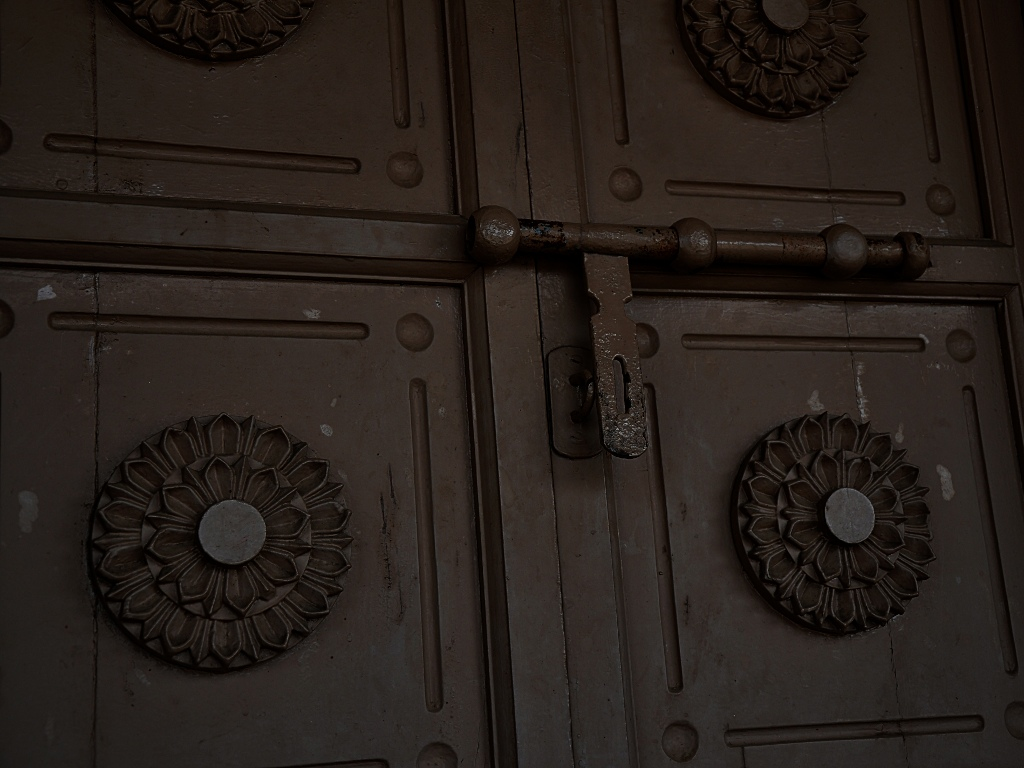
\includegraphics[width=\paperwidth]{images/bg}}
\usecolortheme{albatross}

%% Begin the doc
\begin{document}

%% Title prepare
\color{white}
\title{ತೆರೆಯಲ್ಲಿ ಸುಂದರ ಅಕ್ಷರಗಳು - ಒಂದು ಕಿರುಪರಿಚಯ}
\author{\color{yellow}ಹಳ್ಳಿಮನೆ ಅರವಿಂದ \\ \url{http://aravindavk.in}}
\date{ಜನವರಿ ೨೨, ೨೦೧೨}

\begin{spacing}{1.6}
  %% Slide 0
  \begin{frame}
    \maketitle
  \end{frame}

  %% Slide 1
  \begin{frame}
    \frametitle{ಫಾಂಟ್ ಒಳಗೆ ಏನಿದೆ?}
    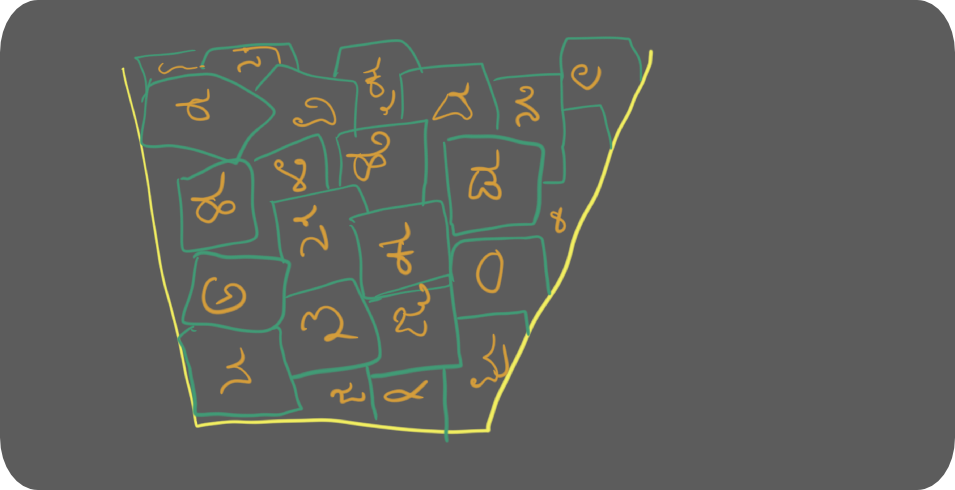
\includegraphics[width=\textwidth]{images/without-tags-bg.png}
  \end{frame}

  %% Slide 2
  \begin{frame}
    \frametitle{ಚಿತ್ರಗಳಿಗೆ ಹೆಸರಿದ್ದರೆ ಸುಲಭವಲ್ಲವೇ?}
    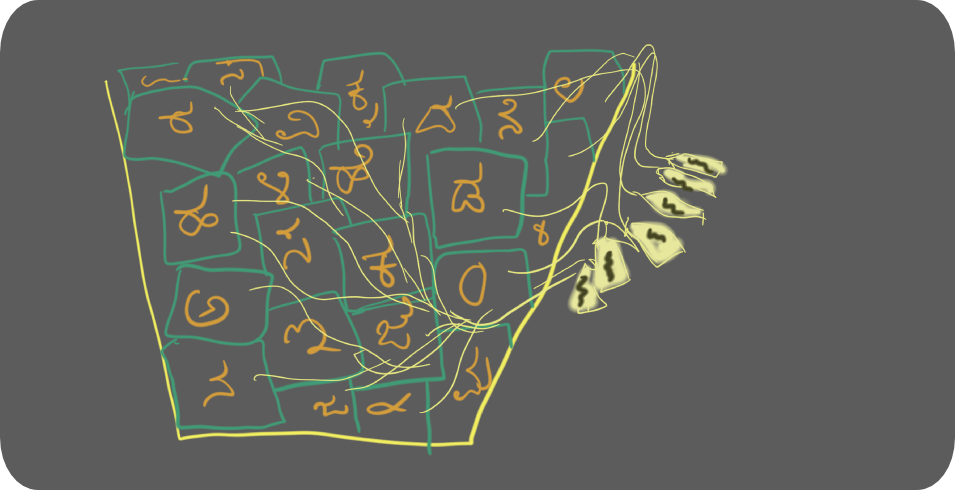
\includegraphics[width=\textwidth]{images/with-tags-bg.png}
  \end{frame}

  %% Slide 3
  \begin{frame}
    \frametitle{ಎಲ್ಲಾ ಚಿತ್ರಕ್ಕೂ ಒಂದೊಂದು ಹೆಸರಿಡಲು ಸಾಧ್ಯವೇ?}
    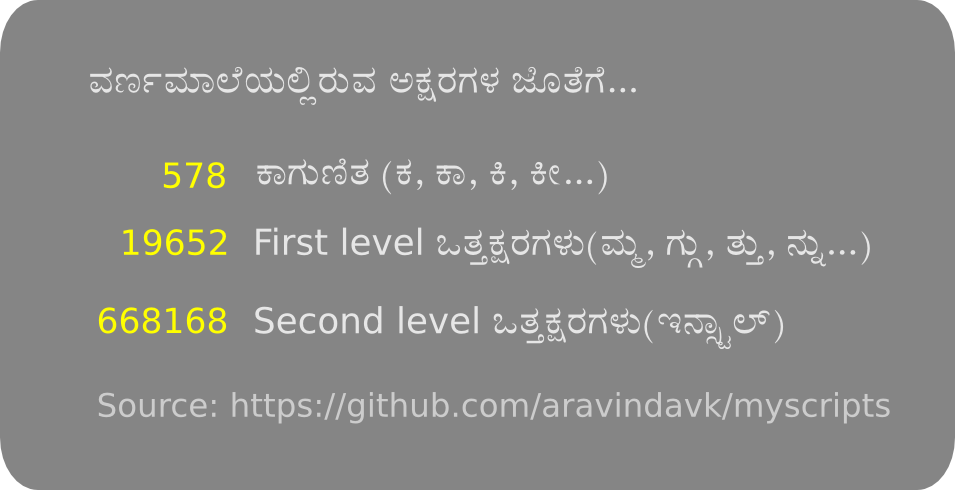
\includegraphics[width=\textwidth]{images/stats.png}
  \end{frame}

  %% Slide 4
  \begin{frame}
    \frametitle{\en{ASCII}}
    \begin{itemize}
    \item \en{The American Standard Code for Information Interchange}
    \item \en{128 characters limit}
    \item ವಿವಿಧ ಭಾಷೆಗಳನ್ನು ಒಟ್ಟೊಟ್ಟಿಗೆ ಬಳಸುವುದು ಕಷ್ಟ.
    \item ಅದನ್ನು ಬರೆಯುವಾಗ ಉಪಯೋಗಿಸಿದ ಫಾಂಟ್ ಇಲ್ಲದಿದ್ದರೆ ಓದುವುದು ಕಷ್ಟ.
    \end{itemize}
  \end{frame}

  %% Slide 5
  \begin{frame}
    \frametitle{\en{Unicode}}
    \begin{itemize}
    \item \en{characters limit} ಇಲ್ಲ.
    \item ಪ್ರಪಂಚದ ಎಲ್ಲಾ ಭಾಷೆಗಳಿಗೂ \en{support} ಇದೆ.
    \item ಅದೇ ಭಾಷೆಯ ಯಾವುದೇ ಫಾಂಟ್ ಇದ್ದರೂ ಓದಬಹುದು.

    \end{itemize}
  \end{frame}

  %% Slide 6
  \begin{frame}
    \frametitle{\en{ASCII vs Unicode}}
    \begin{columns}[t]
      \column{5cm}
      \LARGE{\en{ASCII}} \\
      \normalsize \en{gÉÆ} ``ರೊ'' ಬರೆಯಲು ಮೂರು ಅಕ್ಷರಗಳು ಬೇಕು.
      \column{5cm}
      \LARGE{\en{Unicode}} \\
      \normalsize ರ +  ೊ  = ``ರೊ'' ಬರೆಯಲು ಎರಡು ಅಕ್ಷರಗಳು ಸಾಕು.
    \end{columns}
  \end{frame}

  %% Slide 7
  \begin{frame}
    \frametitle{ಒಂದೊಂದು ಚಿತ್ರಗಳೂ ಹೇಗಿರಬೇಕು?}
    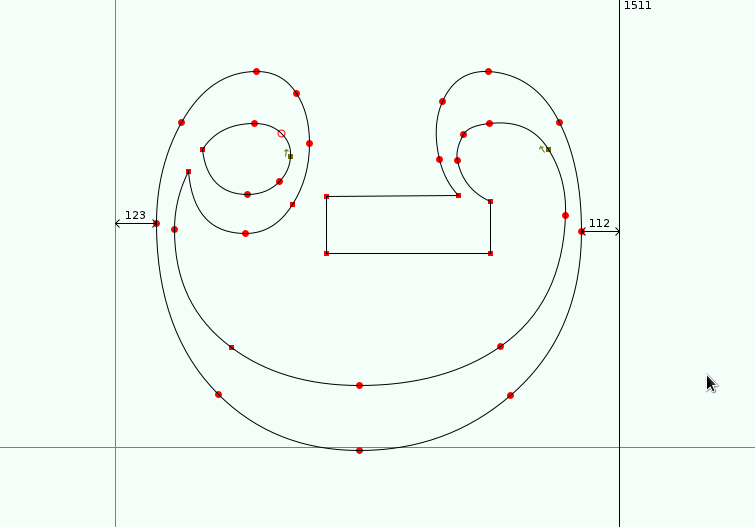
\includegraphics[width=\textwidth]{images/aglyph.png}
  \end{frame}

  %% Slide 8
  \begin{frame}
    \frametitle{ಚಿತ್ರಗಳನ್ನು ಹೀಗೆ ಜೋಡಿಸಿದರೆ ಸಾಕೆ?}
    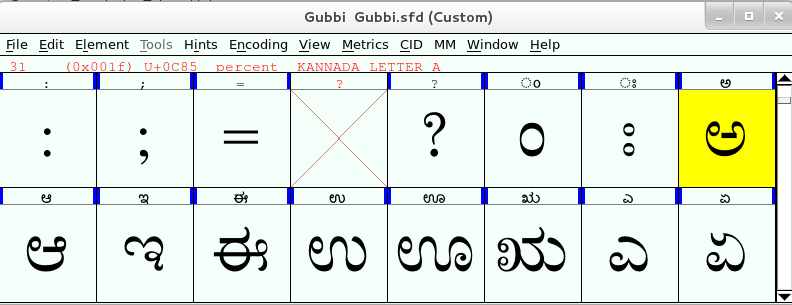
\includegraphics[width=\textwidth]{images/glyphs.png}
  \end{frame}

  %% Slide 9
  \begin{frame}
    \frametitle{ನಿಯಮಗಳು, ಉದಾಹರಣೆ ೧}
    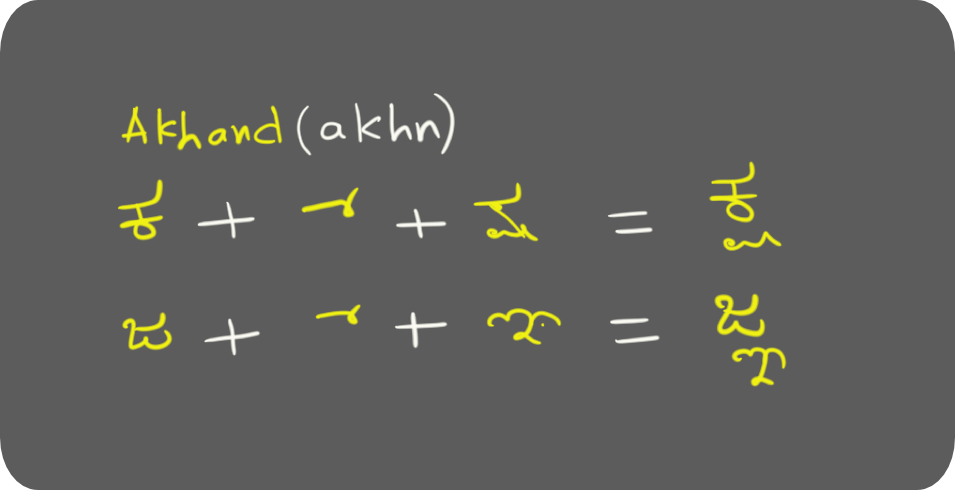
\includegraphics[width=\textwidth]{images/akhn-bg.png}
  \end{frame}

  %% Slide 10
  \begin{frame}
    \frametitle{ನಿಯಮಗಳು, ಉದಾಹರಣೆ ೨}
    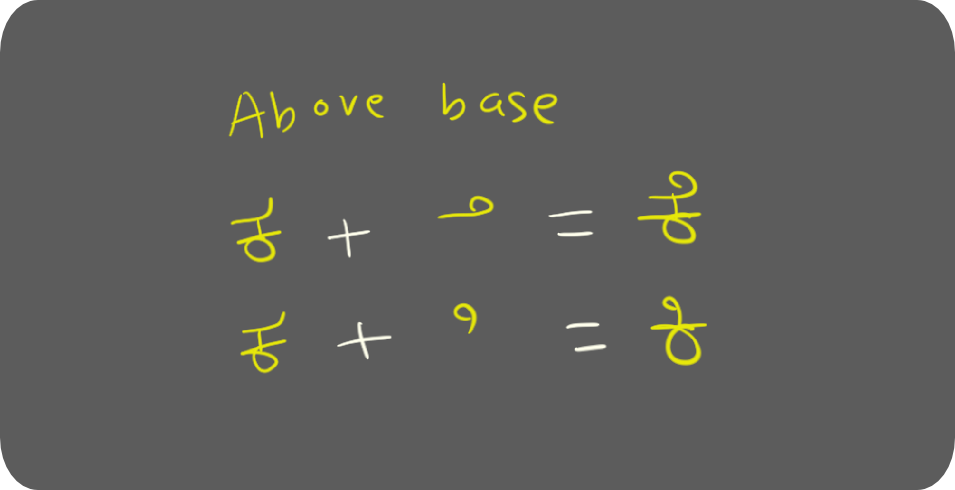
\includegraphics[width=\textwidth]{images/abvs-bg.png}
  \end{frame}

  %% Slide 11
  \begin{frame}
    \frametitle{ನಿಯಮಗಳು, ಉದಾಹರಣೆ ೩}
    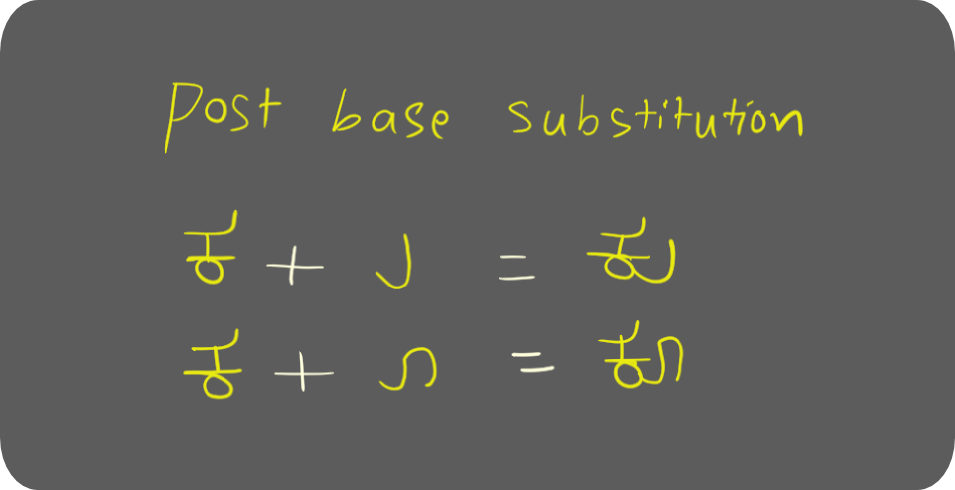
\includegraphics[width=\textwidth]{images/psts-bg.png}
  \end{frame}

  %% Slide 12
  \begin{frame}
    \frametitle{\en{Typography}}
    \begin{itemize}
    \item ಅಕ್ಷರಗಳ ಎತ್ತರ.
    \item ಅಕ್ಷರಗಳ ದಪ್ಪ.
    \item ಎರಡು ಅಕ್ಷರಗಳ ನಡುವಿನ ಅಂತರ.
    \item ಸುಂದರ ಆಕೃತಿಗಳು.
    \end{itemize}
  \end{frame}

  %% Slide 13
  \begin{frame}
    \frametitle{\en{License}}
    ಮುಕ್ತ ಲೈಸೆನ್ಸ್ ಗಳು, ಉದಾ: \en{OFL Open Font License}
  \end{frame}

  %% Slide 14
  \begin{frame}
    \frametitle{ತಂತ್ರಾಂಶಗಳು ಯಾವುದಿವೆ?}
    \begin{itemize}
    \item \en{FontForge} \url{http://fontforge.sourceforge.net}
    \item \en{FontForge Python} \url{http://fontforge.sourceforge.net/python.html}
    \item \en{Inkscape} \url{http://inkscape.org/}
    \item \en{MetaPost} \url{http://www.tug.org/metapost.html}
    \end{itemize}
  \end{frame}

  %% Slide 15
  \begin{frame}
    \frametitle{ಗುಬ್ಬಿ ಮತ್ತು ನವಿಲು}
    \begin{columns}[t]
      \column{5cm}
      
\includegraphics[width=\textwidth]{images/gubbi-showcase.png} \\
      \LARGE{ಗುಬ್ಬಿ}

      \normalsize \url{https://github.com/aravindavk/Gubbi}
      \column{5cm}
      
\includegraphics[width=\textwidth]{images/navilu-showcase.png} \\
      \LARGE{ನವಿಲು}

      \normalsize \url{https://github.com/aravindavk/Navilu}
    \end{columns}
  \end{frame}
  %% Slide 16
  \begin{frame}
    \frametitle{ಕುತೂಹಲವಿದ್ದಷ್ಟೂ ಒಳ್ಳೆಯದು, ಬಾಗಿಲು ತೆರೆದು ಒಳಗೇನಿದೆ ನೋಡೋಣ ಬನ್ನಿ...}
    \LARGE
    ಪ್ರಶ್ನೆಗಳು? \\
    \vspace{0.6in}
    ಸಂಪರ್ಕಿಸಿ:
    \footnotesize
    \begin{spacing}{1.2}
    \begin{itemize}
    \item \en{Website: } \url{http://aravindavk.in}
    \item \en{Twitter: } \href{http://twitter.com/aravindavk}{\en{@aravindavk}}
    \item \en{Github: } \url{http://github.com/aravindavk}
    \item \en{Email: }\href{mailto:hallimanearavind@gmail.com}{\en{hallimanearavind@gmail.com}}
    \end{itemize}
    \end{spacing}
   

  \end{frame}
  \end{spacing}

\end{document}
